\section{Räuber und Beute}
\begin{code}
	\caption{Skript für die kontinuierliche Berechnung des Verlaufs}
	\mSourceFile{\srcDir/predatorPrey.m}
	\label{source:3-script}
\end{code}
\ \newpage
\begin{figure}[h]
	\centering
	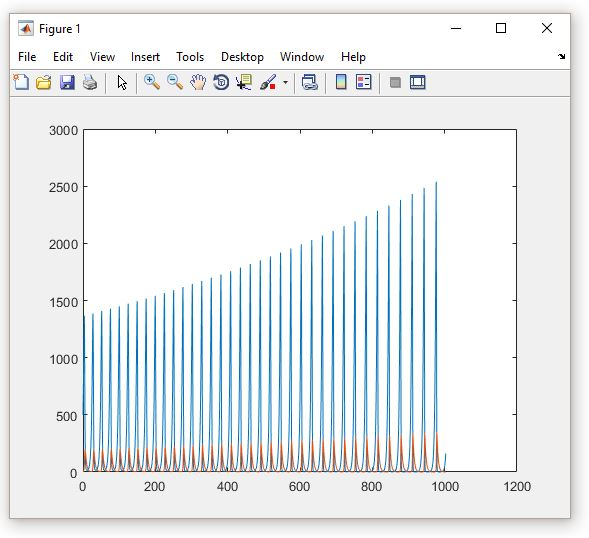
\includegraphics[scale=1]{\imageDir/4-test.JPG}
	\caption{Verlauf P,B über t}
	\label{fig:3-test-1}
\end{figure}
\ \newpage
\begin{figure}[h]
\centering
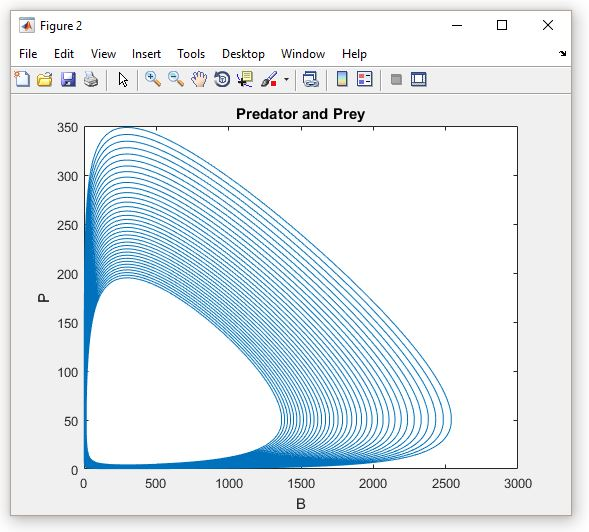
\includegraphics[scale=1]{\imageDir/4-test-1.JPG}
\caption{Verlauf P über B}
\label{fig:3-test-2}
\end{figure}